% !TEX program = xelatex
% Defensa de propuesta de tesis. Diapositivas 1 a 3 (portada, agenda, contexto).
% Compilador: XeLaTeX (el tema Metropolis usa la fuente Fira Sans).
\documentclass[aspectratio=169,11pt]{beamer}

\usetheme[progressbar=frametitle,numbering=fraction]{metropolis}
\usepackage[spanish,es-noshorthands]{babel}
\usepackage{graphicx}
\usepackage{xcolor}

% Colores: azul sobrio y un acento dorado (piña)
\definecolor{tecblue}{HTML}{1B365D}
\definecolor{pina}{HTML}{B87A00}
\setbeamercolor{frametitle}{bg=tecblue,fg=white}
\setbeamercolor{progress bar}{fg=pina,bg=tecblue!25}
\setbeamercolor{alerted text}{fg=pina}
\setbeamercolor{block title alerted}{bg=tecblue!10,fg=tecblue}
\setbeamercolor{block body alerted}{bg=tecblue!5,fg=black}
\setbeamercolor{title separator}{fg=pina}

% Portada
\title{Effect of Data Processing and VAE Modifications on Latent Diffusion Image Generation with a Small Homogeneous UAV Dataset: A Case Study on Pineapple Fields}
\subtitle{Defensa de propuesta de tesis \textbullet{} Seminario de investigación 1}
\author{Oscar Daniel Ortega Navarro\\[2pt]\footnotesize Asesor: Fabián Fallas Moya}
\institute{Instituto Tecnológico de Costa Rica\\ Escuela de Ciencias de la Computación \textbullet{} Programa de Maestría en Computación}
\date{Miércoles 25 de noviembre de 2026}
\titlegraphic{\hfill
\includegraphics[height=1.1cm]{Imagenes/logo.png}}

\setbeamerfont{title}{size=\large}
\setbeamerfont{subtitle}{size=\normalsize}

\begin{document}

% ---------------------------------------------------------------- 1. Portada
\maketitle

% ---------------------------------------------------------------- 2. Agenda
\begin{frame}{Agenda}
  \begin{columns}[T]
    \begin{column}{0.48\textwidth}
      \begin{enumerate}
        \setlength\itemsep{4pt}
        \item Contexto
        \item Problema, justificación y vacío de investigación
        \item Descripción del proyecto
        \item Pregunta de investigación e hipótesis
        \item Objetivos
      \end{enumerate}
    \end{column}
    \begin{column}{0.48\textwidth}
      \begin{enumerate}
        \setcounter{enumi}{5}
        \setlength\itemsep{4pt}
        \item Evidencia preliminar
        \item Metodología y flujo estadístico
        \item Métricas y entregables
        \item Cronograma y riesgos
      \end{enumerate}
    \end{column}
  \end{columns}
\end{frame}

% ---------------------------------------------------------------- 3. Contexto
\begin{frame}{Contar piña desde el aire}
  \begin{columns}[T]
    \begin{column}{0.26\textwidth}
      \centering
      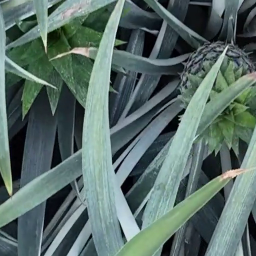
\includegraphics[width=\linewidth]{Imagenes/defensa_cuadro_real.png}\\[2pt]
      {\tiny\color{gray} Cuadro real del conjunto de datos}
    \end{column}
    \begin{column}{0.72\textwidth}
      \small
      \textbf{\color{tecblue}Por qué contar}\\
      Cuántas plantas hay por hectárea \alert{influye mucho en cuánta fruta se cosecha}. A mano, en áreas grandes, no es práctico. \emph{Piña en Costa Rica: +40\,000 ha \textbullet{} 60\,000 a 100\,000 plantas por hectárea.}\\[-1pt]
      {\tiny\color{gray} Kitano et al. (2019) \textbullet{} Castro (2019)}

      \vspace{5pt}
      \textbf{\color{tecblue}Cómo se cuenta con drones}\\
      \alert{Detectores} aplicados a imágenes de dron; en piña se cuentan frutos maduros. El conteo se hace \alert{contando detecciones} o \alert{aprendiendo un mapa de densidad}.\\[-1pt]
      {\tiny\color{gray} Shiu et al. (2023)}

      \vspace{5pt}
      \textbf{\color{tecblue}Qué lo limita}\\
      Los datos: \alert{pocos, parecidos y caros de etiquetar}.\\[-1pt]
      {\tiny\color{gray} González-Hernández et al. (2026) \textbullet{} Bah et al. (2018) \textbullet{} Cai et al. (2022)}
    \end{column}
  \end{columns}

  \vfill
  \begin{alertblock}{Una vía: imágenes sintéticas}
    \small Ya mejoraron la detección y el conteo en otros cultivos (sorgo, vid). \alert{Esta propuesta estudia cómo generarlas bien}; no entrena el contador.
    {\tiny\color{gray}\hfill Cai et al. (2022) \textbullet{} Hirahara et al. (2025)}
  \end{alertblock}
\end{frame}

% ---------------------------------------------------------------- (siguientes diapositivas)

\end{document}
